% Options for packages loaded elsewhere
% Options for packages loaded elsewhere
\PassOptionsToPackage{unicode}{hyperref}
\PassOptionsToPackage{hyphens}{url}
%
\documentclass[
  ignorenonframetext,
  aspectratio=169,
]{beamer}
\newif\ifbibliography
\usepackage{pgfpages}
\setbeamertemplate{caption}[numbered]
\setbeamertemplate{caption label separator}{: }
\setbeamercolor{caption name}{fg=normal text.fg}
\beamertemplatenavigationsymbolsempty
% remove section numbering
\setbeamertemplate{part page}{
  \centering
  \begin{beamercolorbox}[sep=16pt,center]{part title}
    \usebeamerfont{part title}\insertpart\par
  \end{beamercolorbox}
}
\setbeamertemplate{section page}{
  \centering
  \begin{beamercolorbox}[sep=12pt,center]{section title}
    \usebeamerfont{section title}\insertsection\par
  \end{beamercolorbox}
}
\setbeamertemplate{subsection page}{
  \centering
  \begin{beamercolorbox}[sep=8pt,center]{subsection title}
    \usebeamerfont{subsection title}\insertsubsection\par
  \end{beamercolorbox}
}
% Prevent slide breaks in the middle of a paragraph
\widowpenalties 1 10000
\raggedbottom
\AtBeginPart{
  \frame{\partpage}
}
\AtBeginSection{
  \ifbibliography
  \else
    \frame{\sectionpage}
  \fi
}
\AtBeginSubsection{
  \frame{\subsectionpage}
}
\usepackage{iftex}
\ifPDFTeX
  \usepackage[T1]{fontenc}
  \usepackage[utf8]{inputenc}
  \usepackage{textcomp} % provide euro and other symbols
\else % if luatex or xetex
  \usepackage{unicode-math} % this also loads fontspec
  \defaultfontfeatures{Scale=MatchLowercase}
  \defaultfontfeatures[\rmfamily]{Ligatures=TeX,Scale=1}
\fi
\usepackage{lmodern}

\ifPDFTeX\else
  % xetex/luatex font selection
\fi
% Use upquote if available, for straight quotes in verbatim environments
\IfFileExists{upquote.sty}{\usepackage{upquote}}{}
\IfFileExists{microtype.sty}{% use microtype if available
  \usepackage[]{microtype}
  \UseMicrotypeSet[protrusion]{basicmath} % disable protrusion for tt fonts
}{}
\makeatletter
\@ifundefined{KOMAClassName}{% if non-KOMA class
  \IfFileExists{parskip.sty}{%
    \usepackage{parskip}
  }{% else
    \setlength{\parindent}{0pt}
    \setlength{\parskip}{6pt plus 2pt minus 1pt}}
}{% if KOMA class
  \KOMAoptions{parskip=half}}
\makeatother


\usepackage{longtable,booktabs,array}
\usepackage{calc} % for calculating minipage widths
\usepackage{caption}
% Make caption package work with longtable
\makeatletter
\def\fnum@table{\tablename~\thetable}
\makeatother
\usepackage{graphicx}
\makeatletter
\newsavebox\pandoc@box
\newcommand*\pandocbounded[1]{% scales image to fit in text height/width
  \sbox\pandoc@box{#1}%
  \Gscale@div\@tempa{\textheight}{\dimexpr\ht\pandoc@box+\dp\pandoc@box\relax}%
  \Gscale@div\@tempb{\linewidth}{\wd\pandoc@box}%
  \ifdim\@tempb\p@<\@tempa\p@\let\@tempa\@tempb\fi% select the smaller of both
  \ifdim\@tempa\p@<\p@\scalebox{\@tempa}{\usebox\pandoc@box}%
  \else\usebox{\pandoc@box}%
  \fi%
}
% Set default figure placement to htbp
\def\fps@figure{htbp}
\makeatother





\setlength{\emergencystretch}{3em} % prevent overfull lines

\providecommand{\tightlist}{%
  \setlength{\itemsep}{0pt}\setlength{\parskip}{0pt}}



 


\makeatletter
\@ifpackageloaded{caption}{}{\usepackage{caption}}
\AtBeginDocument{%
\ifdefined\contentsname
  \renewcommand*\contentsname{Table of contents}
\else
  \newcommand\contentsname{Table of contents}
\fi
\ifdefined\listfigurename
  \renewcommand*\listfigurename{List of Figures}
\else
  \newcommand\listfigurename{List of Figures}
\fi
\ifdefined\listtablename
  \renewcommand*\listtablename{List of Tables}
\else
  \newcommand\listtablename{List of Tables}
\fi
\ifdefined\figurename
  \renewcommand*\figurename{Figure}
\else
  \newcommand\figurename{Figure}
\fi
\ifdefined\tablename
  \renewcommand*\tablename{Table}
\else
  \newcommand\tablename{Table}
\fi
}
\@ifpackageloaded{float}{}{\usepackage{float}}
\floatstyle{ruled}
\@ifundefined{c@chapter}{\newfloat{codelisting}{h}{lop}}{\newfloat{codelisting}{h}{lop}[chapter]}
\floatname{codelisting}{Listing}
\newcommand*\listoflistings{\listof{codelisting}{List of Listings}}
\makeatother
\makeatletter
\makeatother
\makeatletter
\@ifpackageloaded{caption}{}{\usepackage{caption}}
\@ifpackageloaded{subcaption}{}{\usepackage{subcaption}}
\makeatother

\usepackage{bookmark}
\IfFileExists{xurl.sty}{\usepackage{xurl}}{} % add URL line breaks if available
\urlstyle{same}
\hypersetup{
  pdftitle={Análise Discriminante},
  hidelinks,
  pdfcreator={LaTeX via pandoc}}



\title{Análise Discriminante}
\author{}
\date{}

\begin{document}
\frame{\titlepage}


\begin{frame}
\begin{block}{O Problema da classificação e discriminação}
\phantomsection\label{o-problema-da-classificauxe7uxe3o-e-discriminauxe7uxe3o}
\begin{itemize}
\tightlist
\item
  Dois tipos de problemas recorrentes em análise de dados, e que podem
  ser abordados por técnicas multivariadas, são \textbf{discriminação} e
  \textbf{classificação}.
\end{itemize}

\pause

\begin{itemize}
\tightlist
\item
  Em um problema de \textbf{discriminação}, o objetivo é aplicar e
  avaliar a contribuição de \(p\) variáveis na discriminação (separação)
  de \(k\) grupos \textbf{pré-definidos};
\end{itemize}

\pause

\begin{itemize}
\tightlist
\item
  Em um problema de \textbf{classificação}, o objetivo é construir uma
  regra, baseada em \(p\) variáveis e \(n\) indivíduos, que permita
  classificar novos indivíduos em um de \(k\) grupos
  \textbf{pré-definidos}.
\end{itemize}
\end{block}

\begin{block}{Discriminação em dois grupos}
\phantomsection\label{discriminauxe7uxe3o-em-dois-grupos}
\begin{itemize}
\tightlist
\item
  Considere que desejamos discriminar indivíduos de duas populações
  \(\boldsymbol{\pi}_1\) e \(\boldsymbol{\pi}_2\) com base em \(p\)
  variáveis avaliadas \(\boldsymbol{x} = [X_1, X_2, \cdots, X_p]^t\).
\end{itemize}

\pause

\begin{itemize}
\tightlist
\item
  Considere ainda conhecidas \(\boldsymbol{\mu}_1\),
  \(\boldsymbol{\mu}_2\), \(\boldsymbol{\Sigma}_1\) e
  \(\boldsymbol{\Sigma}_2\).
\end{itemize}

\pause

\begin{itemize}
\tightlist
\item
  Sejam \(f_1(\boldsymbol{x})\) e \(f_2(\boldsymbol{x})\) as funções
  (densidade) de probabilidade de \(\boldsymbol{x}\) em
  \(\boldsymbol{\pi}_1\) e \(\boldsymbol{\pi}_2\).
\end{itemize}

\pause

\begin{itemize}
\tightlist
\item
  Seja \(\Omega\) o espaço amostral (conjunto de resultados possíveis
  para \(\boldsymbol{x}\)).
\end{itemize}
\end{block}

\begin{block}{Classificação em dois grupos - Regras de classificação}
\phantomsection\label{classificauxe7uxe3o-em-dois-grupos---regras-de-classificauxe7uxe3o}
\begin{itemize}
\tightlist
\item
  Vamos considerar uma partição de \(\Omega\) em dois conjuntos \(R_1\)
  e \(R_2\), \((R_1 \cup R_2 = \Omega; R_1 \cap R_2 = \emptyset)\), tal
  que:

  \begin{itemize}
  \tightlist
  \item
    Todo indivíduo tal que \(\boldsymbol{x} \in R_1\) seja classificado
    como pertencente a \(\boldsymbol{\pi}_1\);
  \item
    Todo indivíduo tal que \(\boldsymbol{x} \in \Omega - R_1 = R_2\)
    seja classificado como pertencente a \(\boldsymbol{\pi}_2\).
  \end{itemize}
\end{itemize}
\end{block}

\begin{block}{Classificação em dois grupos - Ilustração}
\phantomsection\label{classificauxe7uxe3o-em-dois-grupos---ilustrauxe7uxe3o}
\begin{center}
\pandocbounded{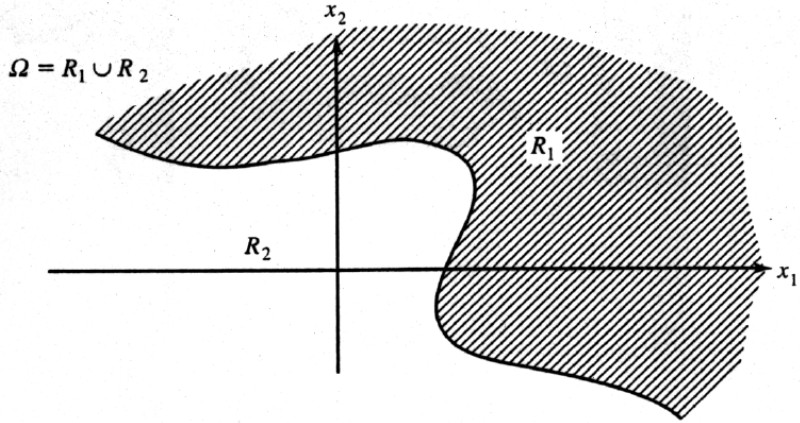
\includegraphics[keepaspectratio]{../../images/AD/discriminacao_2_grupos.jpg}}
\end{center}
\end{block}

\begin{block}{Classificação em dois grupos - Probabilidades de
má-classificação}
\phantomsection\label{classificauxe7uxe3o-em-dois-grupos---probabilidades-de-muxe1-classificauxe7uxe3o}
Com base no que foi apresentado, temos as seguintes probabilidades:

\begin{itemize}
\tightlist
\item
  \(P(2|1)\): Probabilidade de classificar um indivíduo em
  \(\boldsymbol{\pi}_2\) dado que ele pertence a \(\boldsymbol{\pi}_1\):
\end{itemize}

\[\small P(2|1) = P(\boldsymbol{x }\in R_2| \boldsymbol{\pi}_1) = \displaystyle{\int_{R_2} f_1(\boldsymbol{x}) d \boldsymbol{x}}\]

\begin{itemize}
\tightlist
\item
  \(P(1|2)\): Probabilidade de classificar um indivíduo em
  \(\boldsymbol{\pi}_1\) dado que ele pertence a \(\boldsymbol{\pi}_2\):
\end{itemize}

\[\small P(1|2) = P(\boldsymbol{x} \in R_1| \boldsymbol{\pi}_2) = \displaystyle{\int_{R_1} f_2(\boldsymbol{x}) d \boldsymbol{x}}\]
\end{block}

\begin{block}{Classificação em dois grupos - Ilustração}
\phantomsection\label{classificauxe7uxe3o-em-dois-grupos---ilustrauxe7uxe3o-1}
\begin{center}
\pandocbounded{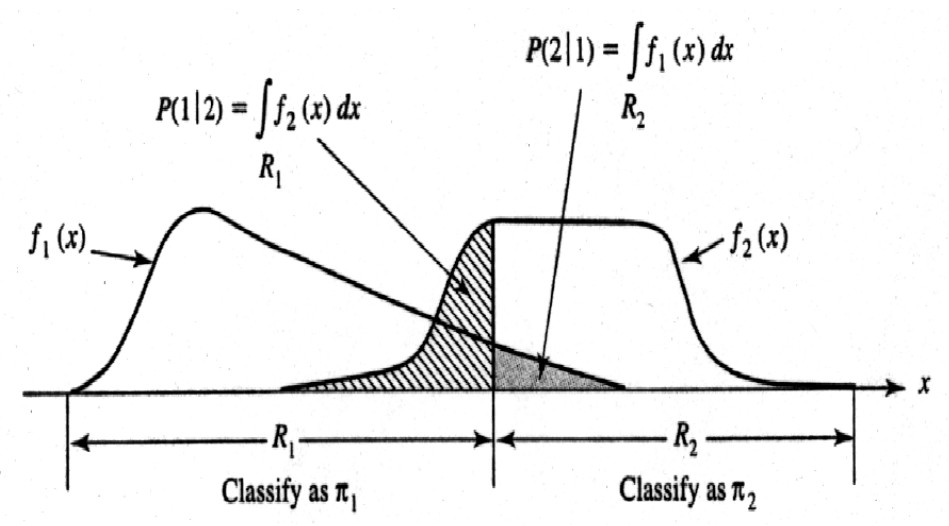
\includegraphics[keepaspectratio]{../../images/AD/prob_ma_class_2_pop.jpg}}
\end{center}
\end{block}

\begin{block}{Classificação em dois grupos - Incorporando probabilidades
a priori}
\phantomsection\label{classificauxe7uxe3o-em-dois-grupos---incorporando-probabilidades-a-priori}
Vamos assumir probabilidades a priori \(p_1 = P(\boldsymbol{\pi}_1)\) e
\(p_2 = P(\boldsymbol{\pi}_2)\) de um indivíduo pertencer a
\(\boldsymbol{\pi}_1\) e \(\boldsymbol{\pi}_2\), respectivamente
(\(p_1 + p_2 = 1\)). Então:

\begin{itemize}
\tightlist
\item
  Probabilidade de um indivíduo ser classificado na população 1
  (\(C_1\)) e de fato pertencer a \(\boldsymbol{\pi}_1\):
\end{itemize}

\[P(C_1 \cap \boldsymbol{\pi}_1) = P(C_1|\boldsymbol{\pi}_1)P(\boldsymbol{\pi}_1) = P(1|1)p_1\]

\begin{itemize}
\tightlist
\item
  Probabilidade de um indivíduo ser incorretamente classificado na
  população \(\boldsymbol{\pi}_1\):
\end{itemize}

\[P(C_1 \cap \boldsymbol{\pi}_2) = P(C_1|\boldsymbol{\pi}_2)P(\boldsymbol{\pi}_2) = P(1|2)p_2\]
\end{block}

\begin{block}{Classificação em dois grupos - Incorporando probabilidades
a priori}
\phantomsection\label{classificauxe7uxe3o-em-dois-grupos---incorporando-probabilidades-a-priori-1}
\begin{itemize}
\tightlist
\item
  Probabilidade de um indivíduo ser classificado na população 2
  (\(C_2\)) e de fato pertencer a \(\boldsymbol{\pi}_2\):
\end{itemize}

\[P(C_2 \cap \boldsymbol{\pi}_2) = P(C_2|\boldsymbol{\pi}_2)P(\boldsymbol{\pi}_2) = P(2|2)p_2\]

\begin{itemize}
\tightlist
\item
  Probabilidade de um indivíduo ser incorretamente classificado na
  população \(\boldsymbol{\pi}_2\):
\end{itemize}

\[P(C_2 \cap \boldsymbol{\pi}_1) = P(C_2|\boldsymbol{\pi}_1)P(\boldsymbol{\pi}_1) = P(2|1)p_1\]
\end{block}

\begin{block}{Classificação em dois grupos - Incorporando custos de
má-classificação}
\phantomsection\label{classificauxe7uxe3o-em-dois-grupos---incorporando-custos-de-muxe1-classificauxe7uxe3o}
Agora vamos incorporar custos de má-classificação:

\begin{itemize}
\tightlist
\item
  Seja \(c(1|2)\) o custo de classificar um indivíduo pertencente a
  \(\boldsymbol{\pi}_2\) como pertencente a \(\boldsymbol{\pi}_1\);
\end{itemize}

\pause

\begin{itemize}
\tightlist
\item
  Seja \(c(2|1)\) o custo de classificar um indivíduo pertencente a
  \(\boldsymbol{\pi}_1\) como pertencente a \(\boldsymbol{\pi}_2\);
\end{itemize}

\pause

Naturalmente, consideramos \(c(1|1) = c(2|2) = 0\).
\end{block}

\begin{block}{Classificação em dois grupos - Custo esperado de
má-classificação (\(ECM\))}
\phantomsection\label{classificauxe7uxe3o-em-dois-grupos---custo-esperado-de-muxe1-classificauxe7uxe3o-ecm}
Diferentes critérios podem ser utilizados para fins de determinar a
regra de classificação. Um deles é a minimização do \textbf{custo
esperado de má-classificação}.

\begin{itemize}
\tightlist
\item
  Para qualquer regra de classificação, o custo esperado de
  má-classificação (\(ECM\)) fica dado por:
\end{itemize}

\[ECM = c(2|1)P(2|1)p_1 + c(1|2)P(1|2)p_2\]

\begin{itemize}
\tightlist
\item
  Assim, a melhor regra de classificação, baseada nesse critério, seria
  aquela que minimizasse \(ECM\).
\end{itemize}
\end{block}

\begin{block}{Classificação em dois grupos - Regras de classificação
para mínimo (\(ECM\))}
\phantomsection\label{classificauxe7uxe3o-em-dois-grupos---regras-de-classificauxe7uxe3o-para-muxednimo-ecm}
As regiões \(R_1\) e \(R_2\), responsáveis por alocar qualquer
observação \(\boldsymbol{x}\) a \(\boldsymbol{\pi}_1\) ou
\(\boldsymbol{\pi}_2\) (respectivamente), \textbf{tal que \(ECM\) seja
mínimo}, são dadas por:

\[\small R_1: = \dfrac{f_1(\boldsymbol{x})}{f_2(\boldsymbol{x})} \geqslant \left( \dfrac{c(1|2)}{c(2|1)}\right) \left( \dfrac{p_2}{p_1}\right)\]

ou, de forma equivalente,
\(p_1c(2|1)f_1(\boldsymbol{x}) \geqslant p_2c(1|2)f_2(\boldsymbol{x})\);

\[\small R_2: = \dfrac{f_1(\boldsymbol{x})}{f_2(\boldsymbol{x})} < \left( \dfrac{c(1|2)}{c(2|1)}\right) \left( \dfrac{p_2}{p_1}\right)\]

ou, de forma equivalente,
\(p_1c(2|1)f_1(\boldsymbol{x}) < p_2c(1|2)f_2(\boldsymbol{x})\).
\end{block}

\begin{block}{Classificação em dois grupos - casos particulares}
\phantomsection\label{classificauxe7uxe3o-em-dois-grupos---casos-particulares}
\begin{itemize}
\tightlist
\item
  \(p_1 = p_2\) (probabilidades a priori iguais):
\end{itemize}

\[\small R_1: = \dfrac{f_1(\boldsymbol{x})}{f_2(\boldsymbol{x})} \geqslant \left( \dfrac{c(1|2)}{c(2|1)}\right) \,\,\,\,\,\, R_2: = \dfrac{f_1(\boldsymbol{x})}{f_2(\boldsymbol{x})} < \left( \dfrac{c(1|2)}{c(2|1)}\right)\]

\begin{itemize}
\tightlist
\item
  \(c(1|2) = c(2|1)\) (custos de má-classificação iguais):
\end{itemize}

\[\small R_1: = \dfrac{f_1(\boldsymbol{x})}{f_2(\boldsymbol{x})} \geqslant \left( \dfrac{p_2}{p_1}\right) \,\,\,\,\,\, R_2: = \dfrac{f_1(\boldsymbol{x})}{f_2(\boldsymbol{x})} < \left( \dfrac{p_2}{p_1}\right)\]
\end{block}

\begin{block}{Classificação em dois grupos - casos particulares}
\phantomsection\label{classificauxe7uxe3o-em-dois-grupos---casos-particulares-1}
\begin{itemize}
\tightlist
\item
  \(p_1 = p_2\) e \(c(1|2) = c(2|1)\):
\end{itemize}

\[\small R_1: = \dfrac{f_1(\boldsymbol{x})}{f_2(\boldsymbol{x})} \geqslant 1 \,\,\,\,\,\, R_2: = \dfrac{f_1(\boldsymbol{x})}{f_2(\boldsymbol{x})} < 1\]
\end{block}

\begin{block}{Classificação em dois grupos - Classificação pelo Teorema
de Bayes}
\phantomsection\label{classificauxe7uxe3o-em-dois-grupos---classificauxe7uxe3o-pelo-teorema-de-bayes}
Usando o teorema de Bayes, podemos alocar uma nova observação
\(\boldsymbol{x}_0\) à população com maior probabilidade a posteriori:

\[P(\boldsymbol{\pi}_1|\boldsymbol{x}_0) = \dfrac{p_1f_1(\boldsymbol{x}_0)}{p_1f_1(\boldsymbol{x}_0) + p_2f_2(\boldsymbol{x}_0)};\]

\[P(\boldsymbol{\pi}_2|\boldsymbol{x}_0) = 1 - P(\boldsymbol{\pi}_1|\boldsymbol{x}_0)\]
\end{block}

\begin{block}{Classificação em duas população normais}
\phantomsection\label{classificauxe7uxe3o-em-duas-populauxe7uxe3o-normais}
\begin{block}{1º caso: as populações possuem variância comum}
\phantomsection\label{uxba-caso-as-populauxe7uxf5es-possuem-variuxe2ncia-comum}
\begin{itemize}
\tightlist
\item
  Suponha agora que \(\boldsymbol{x}\) segue a distribuição normal
  multivariada. Assim, temos que
\end{itemize}

\[f_i(\boldsymbol{x}) = \left( 2\pi\right) ^{-p/2}\left| \boldsymbol{\Sigma} \right| ^{-1/2} \exp\left\lbrace -\dfrac{1}{2} \left( \boldsymbol{x} - \boldsymbol{\mu}_i\right) ^t \boldsymbol{\Sigma}^{-1} \left( \boldsymbol{x} - \boldsymbol{\mu}_i\right) \right\rbrace \]

para \(i = 1,2\) em que \(\boldsymbol{\mu}_i\) é o vetor de médias da
\(i\)-ésima população e \(\boldsymbol{\Sigma}\) é a matriz de
covariâncias positiva definida comum às duas populações.
\end{block}
\end{block}

\begin{block}{Classificação em duas população normais}
\phantomsection\label{classificauxe7uxe3o-em-duas-populauxe7uxe3o-normais-1}
\begin{block}{1º caso: as populações possuem variância comum}
\phantomsection\label{uxba-caso-as-populauxe7uxf5es-possuem-variuxe2ncia-comum-1}
\begin{itemize}
\tightlist
\item
  De acordo com a regra do mínimo custo esperado de má-classificação
  \((ECM)\), devemos classificar \(\boldsymbol{x}\) em
  \(\boldsymbol{\pi}_1\) se
\end{itemize}

\[\small \dfrac{f_1(\boldsymbol{x})}{f_2(\boldsymbol{x})} \geqslant \left( \dfrac{c(1|2)}{c(2|1)}\right) \left( \dfrac{p_2}{p_1}\right)\]

\begin{itemize}
\tightlist
\item
  Se substituirmos as densidades \(f_1(\boldsymbol{x})\) e
  \(f_2 (\boldsymbol{x})\) pela densidade normal correspondente teremos:
\end{itemize}

\[\small \exp\left\lbrace -\dfrac{1}{2} \left( \boldsymbol{x} - \boldsymbol{\mu}_1\right) ^t \boldsymbol{\Sigma}^{-1} \left( \boldsymbol{x} - \boldsymbol{\mu}_1\right) + \dfrac{1}{2} \left( \boldsymbol{x} - \boldsymbol{\mu}_2\right) ^t \boldsymbol{\Sigma}^{-1} \left( \boldsymbol{x} - \boldsymbol{\mu}_2\right)\right\rbrace \geqslant \left( \dfrac{c(1|2)}{c(2|1)}\right) \left( \dfrac{p_2}{p_1}\right)\]
\end{block}
\end{block}

\begin{block}{Classificação em duas população normais}
\phantomsection\label{classificauxe7uxe3o-em-duas-populauxe7uxe3o-normais-2}
\begin{block}{1º caso: as populações possuem variância comum}
\phantomsection\label{uxba-caso-as-populauxe7uxf5es-possuem-variuxe2ncia-comum-2}
\begin{itemize}
\tightlist
\item
  Que, depois de algum algebrismo, torna-se
\end{itemize}

\[\small \exp\left\lbrace \left( \boldsymbol{\mu}_1 - \boldsymbol{\mu}_2\right) ^t \boldsymbol{\Sigma}^{-1}\boldsymbol{x} - \dfrac{1}{2} \left( \boldsymbol{\mu}_1 - \boldsymbol{\mu}_2\right) ^t \boldsymbol{\Sigma}^{-1} \left( \boldsymbol{\mu}_1 + \boldsymbol{\mu}_2\right) \right\rbrace \geqslant \left( \dfrac{c(1|2)}{c(2|1)}\right) \left( \dfrac{p_2}{p_1}\right)\]

\begin{itemize}
\tightlist
\item
  Como ambos os termos são positivos, podemos tomar o logaritmo
  preservando a ordem da desigualdade. Assim, devemos alocar
  \(\boldsymbol{x}\) em \(\boldsymbol{\pi}_1\) se
\end{itemize}

\[\small \left( \boldsymbol{\mu}_1 - \boldsymbol{\mu}_2\right) ^t \boldsymbol{\Sigma}^{-1}\boldsymbol{x} - \dfrac{1}{2} \left( \boldsymbol{\mu}_1 - \boldsymbol{\mu}_2\right) ^t \boldsymbol{\Sigma}^{-1} \left( \boldsymbol{\mu}_1 + \boldsymbol{\mu}_2\right) \geqslant \ln \left\lbrace  \left( \dfrac{c(1|2)}{c(2|1)}\right) \left( \dfrac{p_2}{p_1}\right) \right\rbrace \]

e em \(\boldsymbol{\pi}_2\), caso contrário.
\end{block}
\end{block}

\begin{block}{Classificação em duas população normais}
\phantomsection\label{classificauxe7uxe3o-em-duas-populauxe7uxe3o-normais-3}
\begin{block}{Para dados amostrais}
\phantomsection\label{para-dados-amostrais}
Se considerarmos \(n_1\) observações \(p\)-variadas
\(X_{11}, X_{12}, \cdots, X_{1n_1}\) amostradas da população
\(\boldsymbol{\pi}_1\) e \(n_2\), \(X_{21}, X_{22}, \cdots, X_{2n_2}\)
amostradas da população \(\boldsymbol{\pi}_2\), com
\(n_1 + n_2 - 2 \geqslant p\), então a regra de alocação estimada que
minimiza o custo médio de má-classificação é dada por: alocar
\(\boldsymbol{x}\) na população \(\boldsymbol{\pi}_1\) se

\[(\bar{\boldsymbol{x}}_1 - \bar{\boldsymbol{x}}_2)^t \boldsymbol{S}_c^{-1} \boldsymbol{x} - \dfrac{1}{2} (\bar{\boldsymbol{x}}_1 - \bar{\boldsymbol{x}}_2)^t \boldsymbol{S}_c^{-1} (\bar{\boldsymbol{x}}_1 + \bar{\boldsymbol{x}}_2)\geqslant \ln \left\lbrace  \left( \dfrac{c(1|2)}{c(2|1)}\right) \left( \dfrac{p_2}{p_1}\right) \right\rbrace\]

em que

\[\boldsymbol{S}_c =  \displaystyle{\frac{(n_1 - 1) {\boldsymbol{S}_1} + (n_2 - 1) {\boldsymbol{S}_2}}{n_1 + n_2 - 2}}\]
\end{block}
\end{block}

\begin{block}{Classificação em duas população normais}
\phantomsection\label{classificauxe7uxe3o-em-duas-populauxe7uxe3o-normais-4}
\begin{block}{2º caso: as populações não possuem variância comum}
\phantomsection\label{uxba-caso-as-populauxe7uxf5es-nuxe3o-possuem-variuxe2ncia-comum}
Sob a suposição de homogeneidade das matrizes de covariâncias,
verificamos que as regras de classificação originadas foram simples e
lineares.

\begin{itemize}
\tightlist
\item
  Se considerarmos a situação geral em que \(f_1(\boldsymbol{x})\) e
  \(f_2(\boldsymbol{x})\) são modelos normais multivariados com
  parâmetros \(\boldsymbol{\mu}_i\) e \(\boldsymbol{\Sigma}_i\),
  \(i = 1,2\), sendo
  \(\boldsymbol{\Sigma}_1 \neq \boldsymbol{\Sigma}_2\), devemos
  classificar \(\boldsymbol{x}\) em \(\boldsymbol{\pi}_1\), se
\end{itemize}

\[-\dfrac{1}{2} \boldsymbol{x}^t \left( \boldsymbol{\Sigma}_1 - \boldsymbol{\Sigma}_2\right) \boldsymbol{x} + \left( \boldsymbol{\mu}_1^t \boldsymbol{\Sigma}_1^{-1} - \boldsymbol{\mu}_2^t \boldsymbol{\Sigma}_2^{-1}\right) \boldsymbol{x} - \delta \geqslant \ln \left\lbrace  \left( \dfrac{c(1|2)}{c(2|1)}\right) \left( \dfrac{p_2}{p_1}\right) \right\rbrace\]

e em \(\boldsymbol{\pi}_2\), caso contrário.
\end{block}
\end{block}

\begin{block}{Classificação em duas população normais}
\phantomsection\label{classificauxe7uxe3o-em-duas-populauxe7uxe3o-normais-5}
\begin{block}{2º caso: as populações não possuem variância comum}
\phantomsection\label{uxba-caso-as-populauxe7uxf5es-nuxe3o-possuem-variuxe2ncia-comum-1}
\begin{itemize}
\tightlist
\item
  Sendo,
\end{itemize}

\[\delta = \dfrac{1}{2} \ln \left( \dfrac{|\boldsymbol{\Sigma}_1|}{|\boldsymbol{\Sigma}_2|} \right) + \dfrac{1}{2} \left( \boldsymbol{\mu}_1^t \boldsymbol{\Sigma}_1^{-1}\boldsymbol{\mu}_1 - \boldsymbol{\mu}_2^t \boldsymbol{\Sigma}_2^{-1}\boldsymbol{\mu}_2\right) \]

\begin{itemize}
\tightlist
\item
  Ao contrário do caso homocedástico, as regiões de classificação são
  definidas por funções discriminantes quadráticas de
  \(\boldsymbol{x}\).
\end{itemize}
\end{block}
\end{block}

\begin{block}{Classificação em duas população normais}
\phantomsection\label{classificauxe7uxe3o-em-duas-populauxe7uxe3o-normais-6}
\begin{block}{Para dados amostrais}
\phantomsection\label{para-dados-amostrais-1}
\begin{itemize}
\tightlist
\item
  Podemos obter uma regra estimada substituindo os parâmetros
  \(\boldsymbol{\mu}_i\) e \(\boldsymbol{\Sigma}_i\), pelos respectivos
  estimadores \(\bar{\boldsymbol{x}}_i\) e \(\boldsymbol{S}_i\),
  \(i = 1,2\). Assim, devemos alocar \(\boldsymbol{x}\) na população
  \(\boldsymbol{\pi}_1\) se
\end{itemize}

\[-\dfrac{1}{2} \boldsymbol{x}^t \left( \boldsymbol{S}_1 - \boldsymbol{S}_2\right) \boldsymbol{x} + \left( \bar{\boldsymbol{x}}_1^t \boldsymbol{S}_1^{-1} - \bar{\boldsymbol{x}}_2^t \boldsymbol{S}_2^{-1}\right) \boldsymbol{x} - \hat{\delta} \geqslant \ln \left\lbrace  \left( \dfrac{c(1|2)}{c(2|1)}\right) \left( \dfrac{p_2}{p_1}\right) \right\rbrace\]

e em \(\boldsymbol{\pi}_2\), caso contrário, sendo

\[\hat{\delta} = \dfrac{1}{2} \ln \left( \dfrac{|\boldsymbol{S}_1|}{|\boldsymbol{S}_2|} \right) + \dfrac{1}{2} \left( \bar{\boldsymbol{x}}_1^t \boldsymbol{S}_1^{-1}\bar{\boldsymbol{x}}_1 - \bar{\boldsymbol{x}}_2^t \boldsymbol{S}_2^{-1}\bar{\boldsymbol{x}}_2\right)
\]
\end{block}
\end{block}

\begin{block}{Discriminação em duas populações}
\phantomsection\label{discriminauxe7uxe3o-em-duas-populauxe7uxf5es}
\begin{block}{A função discriminante linear de Fisher}
\phantomsection\label{a-funuxe7uxe3o-discriminante-linear-de-fisher}
\begin{itemize}
\tightlist
\item
  Suposição de linearidade: \textbf{Homocedasticidade!}
\end{itemize}

\[\boldsymbol{\Sigma}_1 = \boldsymbol{\Sigma}_2 = \boldsymbol{\Sigma}\]

\begin{itemize}
\item
  Matriz de variância comum
\item
  Não pressupõe normalidade multivariada dos dados!
\end{itemize}
\end{block}
\end{block}

\begin{block}{Discriminação em duas populações}
\phantomsection\label{discriminauxe7uxe3o-em-duas-populauxe7uxf5es-1}
\begin{block}{A função discriminante linear de Fisher}
\phantomsection\label{a-funuxe7uxe3o-discriminante-linear-de-fisher-1}
\begin{itemize}
\tightlist
\item
  Baseada na \textbf{distância de Mahalanobis} entre o indivíduo
  desconhecido \(\boldsymbol{x}_0\) e as médias das populações:
\end{itemize}

\[d^2(\boldsymbol{x}, \boldsymbol{\mu}_i) = (\boldsymbol{x} - \boldsymbol{\mu}_i)^t \boldsymbol{\Sigma}^{-1}(\boldsymbol{x} - \boldsymbol{\mu}_i), \,\,\,\,\, i = 1,2\]

\begin{itemize}
\tightlist
\item
  Intuitivamente, para um novo indivíduo \(\boldsymbol{x}_0\), se
  \(d^2(\boldsymbol{x}_0, \boldsymbol{\mu}_1) < d^2(\boldsymbol{x}_0, \boldsymbol{\mu}_2)\),
  classificamos \(\boldsymbol{x}_0\) em \(\boldsymbol{\pi}_1\). Caso
  contrário, classificamos \(\boldsymbol{x}_0\) em
  \(\boldsymbol{\pi}_2\)
\end{itemize}
\end{block}
\end{block}

\begin{block}{Discriminação em duas populações}
\phantomsection\label{discriminauxe7uxe3o-em-duas-populauxe7uxf5es-2}
\begin{block}{A função discriminante linear de Fisher}
\phantomsection\label{a-funuxe7uxe3o-discriminante-linear-de-fisher-2}
\begin{itemize}
\tightlist
\item
  Expressando essa regra como uma função discriminante:
\end{itemize}

\[
\begin{aligned}
d^2(\boldsymbol{x}, \boldsymbol{\mu}_2) - d^2(\boldsymbol{x}, \boldsymbol{\mu}_1) &= (\boldsymbol{x} - \boldsymbol{\mu}_2)^t \boldsymbol{\Sigma}^{-1}(\boldsymbol{x} - \boldsymbol{\mu}_2) - (\boldsymbol{x} - \boldsymbol{\mu}_1)^t \boldsymbol{\Sigma}^{-1}(\boldsymbol{x} - \boldsymbol{\mu}_1) 
\\  &= (\boldsymbol{\mu}_2 - \boldsymbol{\mu}_1)^t \boldsymbol{\Sigma}^{-1}(\boldsymbol{\mu}_2 + \boldsymbol{\mu}_1) + 2 \boldsymbol{x}^t\boldsymbol{\Sigma}^{-1}(\boldsymbol{\mu}_1 - \boldsymbol{\mu}_2)
\end{aligned}
\]

\begin{itemize}
\tightlist
\item
  A expressão acima pode ser reescrita como:
\end{itemize}

\[ L(\boldsymbol{x}) = \left[ \boldsymbol{x} - \displaystyle{\frac{1}{2}(\boldsymbol{\mu}_1 + \boldsymbol{\mu}_2)} \right]^t \boldsymbol{\Sigma}^{-1}(\boldsymbol{\mu}_1 - \boldsymbol{\mu}_2)\]
\end{block}
\end{block}

\begin{block}{Discriminação em duas populações}
\phantomsection\label{discriminauxe7uxe3o-em-duas-populauxe7uxf5es-3}
\begin{block}{A função discriminante linear de Fisher}
\phantomsection\label{a-funuxe7uxe3o-discriminante-linear-de-fisher-3}
\begin{itemize}
\tightlist
\item
  Ou ainda\ldots{}
\end{itemize}

\[
L(\boldsymbol{x}) = (\boldsymbol{\mu}_1 - \boldsymbol{\mu}_2)^t\boldsymbol{\Sigma}^{-1}\boldsymbol{x} - \displaystyle{\frac{1}{2}(\boldsymbol{\mu}_1 - \boldsymbol{\mu}_2)^t \boldsymbol{\Sigma}^{-1}(\boldsymbol{\mu}_1 + \boldsymbol{\mu}_2)}
\]

\begin{itemize}
\tightlist
\item
  O primeiro termo
\end{itemize}

\[D(\boldsymbol{x}) = (\boldsymbol{\mu}_1 - \boldsymbol{\mu}_2)^t \boldsymbol{\Sigma}^{-1}\boldsymbol{x}\]

é chamado de \textbf{função discriminante linear de Fisher}.
\end{block}
\end{block}

\begin{block}{Discriminação em duas populações}
\phantomsection\label{discriminauxe7uxe3o-em-duas-populauxe7uxf5es-4}
\begin{block}{A função discriminante linear de Fisher}
\phantomsection\label{a-funuxe7uxe3o-discriminante-linear-de-fisher-4}
\begin{itemize}
\tightlist
\item
  Observe o segundo termo de \[
  L(\boldsymbol{x}) = (\boldsymbol{\mu}_1 - \boldsymbol{\mu}_2)^t \boldsymbol{\Sigma}^{-1} \boldsymbol{x} - \displaystyle{\frac{1}{2}(\boldsymbol{\mu}_1 - \boldsymbol{\mu}_2)^t \boldsymbol{\Sigma}^{-1}(\boldsymbol{\mu}_1 + \boldsymbol{\mu}_2)}
  \]
\end{itemize}

após algum algebrismo,

\[
\begin{aligned}
m &= \displaystyle{\frac{1}{2}(\boldsymbol{\mu}_1 - \boldsymbol{\mu}_2)^t \boldsymbol{\Sigma}^{-1}(\boldsymbol{\mu}_1 + \boldsymbol{\mu}_2)} \\ &= 
\displaystyle{\frac{1}{2}} \left[(\boldsymbol{\mu}_1 - \boldsymbol{\mu}_2)^t \boldsymbol{\Sigma}^{-1} \boldsymbol{\mu}_1 + (\boldsymbol{\mu}_1 - \boldsymbol{\mu}_2)^t \boldsymbol{\Sigma}^{-1} \boldsymbol{\mu}_2\right] \\ &=
\displaystyle{\frac{1}{2}} \left[ D(\boldsymbol{\mu}_1) + D(\boldsymbol{\mu}_2) \right] 
\end{aligned}
\]
\end{block}
\end{block}

\begin{block}{Discriminação em duas populações}
\phantomsection\label{discriminauxe7uxe3o-em-duas-populauxe7uxf5es-5}
\begin{block}{A função discriminante linear de Fisher}
\phantomsection\label{a-funuxe7uxe3o-discriminante-linear-de-fisher-5}
\begin{itemize}
\item
  A regra de classificação fica: Se \(D(\boldsymbol{x}_0)  > m\),
  classificamos \(\boldsymbol{x}_0\) em \(\boldsymbol{\pi}_1\). Caso
  contrário, classificamos \(\boldsymbol{x}_0\) em
  \(\boldsymbol{\pi}_2\).
\item
  É interessante observar que
  \((\boldsymbol{\mu}_1 - \boldsymbol{\mu}_2)^t \boldsymbol{\Sigma}^{-1}\boldsymbol{x}\)
  = \(\boldsymbol{b}^t \boldsymbol{x}\), onde
  \(\boldsymbol{b}^t = (\boldsymbol{\mu}_1 - \boldsymbol{\mu}_2)^t \boldsymbol{\Sigma}^{-1}\)
  é um vetor de dimensão \(1 \times p\).
\item
  Desse modo, a \textbf{função discriminante de Fisher} tem a forma:
\end{itemize}

\[(\boldsymbol{\mu}_1 - \boldsymbol{\mu}_2)^t \boldsymbol{\Sigma}^{-1} \boldsymbol{x} = \boldsymbol{b}^t \boldsymbol{x} = b_1x_1 + b_2x_2 + \cdots + b_px_p\]
\end{block}
\end{block}

\begin{block}{Discriminação em duas populações}
\phantomsection\label{discriminauxe7uxe3o-em-duas-populauxe7uxf5es-6}
\begin{block}{Para dados amostrais}
\phantomsection\label{para-dados-amostrais-2}
\[\widehat{D}(\boldsymbol{x}) = (\bar{\boldsymbol{x}}_1 - \bar{\boldsymbol{x}}_2)^tS_c^{-1}\boldsymbol{x}\]
\[\widehat{m} = \displaystyle{\frac{1}{2}} \left[ \widehat{D}( \bar{\boldsymbol{x}}_1) + \widehat{D}(\bar{\boldsymbol{x}}_2) \right]\]

\[\boldsymbol{S}_c =  \displaystyle{\frac{(n_1 - 1) {\boldsymbol{S}_1} + (n_2 - 1) {\boldsymbol{S}_2}}{n_1 + n_2 - 2}}\]
\end{block}
\end{block}

\begin{block}{Probabilidade de classificação incorreta}
\phantomsection\label{probabilidade-de-classificauxe7uxe3o-incorreta}
\begin{block}{Estimação das probabilidades de classificação incorreta}
\phantomsection\label{estimauxe7uxe3o-das-probabilidades-de-classificauxe7uxe3o-incorreta}
\begin{itemize}
\tightlist
\item
  Seja a seguinte tabela:
\end{itemize}

\[\text{Frequências dos erros de classificação}\]

\begin{longtable}[]{@{}llll@{}}
\toprule\noalign{}
População de origem & Classe 1 & Classe 2 & Total \\
\midrule\noalign{}
\endhead
1 & \(n_{11}\) & \(n_{12}\) & \(n_1\) \\
2 & \(n_{21}\) & \(n_{22}\) & \(n_2\) \\
\bottomrule\noalign{}
\end{longtable}

\[n_{ij}: \text{é o número de elementos de } i \text{ classificados em } j\]
\end{block}
\end{block}

\begin{block}{Probabilidade de classificação incorreta}
\phantomsection\label{probabilidade-de-classificauxe7uxe3o-incorreta-1}
\begin{block}{Estimação das probabilidades de classificação incorreta}
\phantomsection\label{estimauxe7uxe3o-das-probabilidades-de-classificauxe7uxe3o-incorreta-1}
\begin{itemize}
\tightlist
\item
  Com base nessas quantidades, podemos estimar as probabilidades de
  ocorrência dos erros 1 e 2 por:
\end{itemize}

\[\widehat{p}(2|1) = \displaystyle{\frac{n_{12}}{n_1}} \hspace{1cm} \textrm{ e } \hspace{1cm} 
\widehat{p}(1|2) = \displaystyle{\frac{n_{21}}{n_2}}\]

\begin{itemize}
\tightlist
\item
  Além disso, podemos estimar a probabilidade global de acerto da função
  discriminante por:
\end{itemize}

\[\widehat{p}(acerto) = \displaystyle{\frac{n_{11} + n_{22}}{n_1 + n_2}}\]
\end{block}
\end{block}

\begin{block}{Probabilidade de classificação incorreta}
\phantomsection\label{probabilidade-de-classificauxe7uxe3o-incorreta-2}
\begin{block}{Estimação das probabilidades de classificação incorreta}
\phantomsection\label{estimauxe7uxe3o-das-probabilidades-de-classificauxe7uxe3o-incorreta-2}
\begin{itemize}
\tightlist
\item
  Podemos também, estimar a taxa de erro aparente (TEA):
\end{itemize}

\[TEA = \displaystyle{\frac{n_{12} + n_{21}}{n_1 + n_2}}\]
\end{block}
\end{block}

\begin{block}{Probabilidade de classificação incorreta}
\phantomsection\label{probabilidade-de-classificauxe7uxe3o-incorreta-3}
\begin{itemize}
\tightlist
\item
  Três métodos de determinação dessas probabilidades:

  \begin{itemize}
  \tightlist
  \item
    \textbf{Método da ressubstituição:} os mesmos dados são utilizados
    para estimar e validar a função discriminante.
  \item
    \textbf{Método da ressubstituição com divisão amostral:} os dados
    são divididos em duas subamostras - treinamento: estima a fd,
    validação: estima as probabilidades de erro.
  \item
    \textbf{Método da validação cruzada:} a cada iteração é omitida uma
    observação e a fd é estimada a partir das demais. A observação
    omitida é utilizada para estimar as probabilidades de erro.
  \end{itemize}
\end{itemize}
\end{block}

\begin{block}{Classificação em \(k\) grupos}
\phantomsection\label{classificauxe7uxe3o-em-k-grupos}
\begin{itemize}
\tightlist
\item
  Sejam
  \(f_1(\boldsymbol{x}), f_2(\boldsymbol{x}), \cdots, f_k(\boldsymbol{x})\)
  as distribuições do vetor aleatório \(\boldsymbol{x}\) em cada uma de
  \(k\) populações,
  \(\boldsymbol{\pi}_1, \boldsymbol{\pi}_2, \cdots, \boldsymbol{\pi}_k\);
\end{itemize}

\pause

\begin{itemize}
\tightlist
\item
  Sejam \(p_1, p_2, \cdots, p_k\) as probabilidades a priori e
  \(c(i|j),\,\,\, i, j = 1, 2, ..., k\), os custos de má-classificação.
\end{itemize}

\pause

\begin{itemize}
\tightlist
\item
  Seja \(R_i\) o conjunto dos \(\boldsymbol{x}'s\) classificados como
  \(\boldsymbol{\pi}_i, \,\,\, i = 1, 2, \cdots, k\), e
\end{itemize}

\[P(j|i) = \displaystyle{\int_{R_j} f_i(\boldsymbol{x}) d\boldsymbol{x}} \,\,\,\, i,j = 1,2, \cdots, k\]
\end{block}

\begin{block}{Classificação em \(k\) grupos}
\phantomsection\label{classificauxe7uxe3o-em-k-grupos-1}
\begin{itemize}
\tightlist
\item
  Custo esperado de má classificação:
\end{itemize}

\[ECM = p_1 ECM(1) + p_2 ECM(2) + \cdots + p_k ECM(k)\]

em que,

\[ECM(i) = P(1|i)c(1|i) + P(2|i)c(2|i) + \cdots + P(k|i)c(k|i), \,\,\, i = 1, 2, \cdots, k\]

\pause

\begin{itemize}
\tightlist
\item
  A regra de classificação \textbf{tal que \(ECM\) seja mínimo} consiste
  em classificar uma observação \(\boldsymbol{x}\) no grupo \(j\) tal
  que:
\end{itemize}

\[\displaystyle{\sum_{i=1, i \neq j}^kp_if_i(\boldsymbol{x})c(j|i)}, \,\,\, \text{seja mínimo.}\]
\end{block}

\begin{block}{Classificação em \(k\) grupos}
\phantomsection\label{classificauxe7uxe3o-em-k-grupos-2}
\begin{itemize}
\tightlist
\item
  Assim, deve-se classificar \(\boldsymbol{x}\) em
  \(\boldsymbol{\pi}_j\) caso a média dos custos de classificações
  incorretas nas demais populações seja mínima.
\end{itemize}

\pause

\begin{itemize}
\tightlist
\item
  Observe que para \(k = 2\) populações, essa regra de classificação
  fica simplificada, sendo dada pela regra de classificação para duas
  populações apresentada anteriormente.
\end{itemize}
\end{block}

\begin{block}{Classificação em mais de duas população normais}
\phantomsection\label{classificauxe7uxe3o-em-mais-de-duas-populauxe7uxe3o-normais}
\begin{itemize}
\tightlist
\item
  Suponha agora que \(\boldsymbol{x}\) segue a distribuição normal
  multivariada. Assim, temos que
\end{itemize}

\[f_i(\boldsymbol{x}) = \left( 2\pi\right) ^{-p/2}\left| \boldsymbol{\Sigma}_i \right| ^{-1/2} \exp\left\lbrace -\dfrac{1}{2} \left( \boldsymbol{x} - \boldsymbol{\mu}_i\right) ^t \boldsymbol{\Sigma}_i^{-1} \left( \boldsymbol{x} - \boldsymbol{\mu}_i\right) \right\rbrace \]

para \(i = 1,2, \cdots, k\) em que \(\boldsymbol{\mu}_i\) é o vetor de
médias da \(i\)-ésima população e \(\boldsymbol{\Sigma}_i\) é a matriz
de covariâncias positiva definida da \(i\)-ésima população.
\end{block}

\begin{block}{Classificação em mais de duas população normais}
\phantomsection\label{classificauxe7uxe3o-em-mais-de-duas-populauxe7uxe3o-normais-1}
\begin{itemize}
\tightlist
\item
  Considerando que estes parâmetros são conhecidos, então pela regra de
  classificação de mínima probabilidade total de classificação
  incorreta, devemos classificar \(\boldsymbol{x}\) na população
  \(\boldsymbol{\pi}_i\) se
\end{itemize}

\[
\begin{aligned}
\ln\left[ p_i f_i(\boldsymbol{x})\right] &= \ln\left( p_i\right) - \dfrac{p}{2} \ln\left( 2 \pi\right) - \dfrac{1}{2} \ln \left( |\boldsymbol{\Sigma}_i|\right) - \dfrac{1}{2} \left( \boldsymbol{x} - \boldsymbol{\mu}_i\right) ^t \boldsymbol{\Sigma}_i^{-1} \left( \boldsymbol{x} - \boldsymbol{\mu}_i\right) \\ &= \max_j \ln\left[ p_j f_j(\boldsymbol{x})\right] 
\end{aligned}  
\]

\begin{itemize}
\tightlist
\item
  Alocamos a observação \(\boldsymbol{x}\) à população que maximiza
  \(\ln\left[ p_j f_j(\boldsymbol{x})\right]\), em relação a todos os
  valores de \(j\), \(j = 1,2, \cdots, k\).
\end{itemize}
\end{block}

\begin{block}{Classificação em mais de duas população normais}
\phantomsection\label{classificauxe7uxe3o-em-mais-de-duas-populauxe7uxe3o-normais-2}
\begin{itemize}
\tightlist
\item
  O termo \(\dfrac{p}{2} \ln\left( 2 \pi\right)\) é constante para todas
  as \(k\) populações e pode ser ignorado.
\end{itemize}

\pause

\begin{itemize}
\tightlist
\item
  O termo resultante é denominado de escore quadrático de discriminação
  e para a \(i\)-ésima população é dado por
\end{itemize}

\[
d_i^Q(\boldsymbol{x}) =  - \dfrac{1}{2} \ln \left( |\boldsymbol{\Sigma}_i|\right) - \dfrac{1}{2} \left( \boldsymbol{x} - \boldsymbol{\mu}_i\right) ^t \boldsymbol{\Sigma}_i^{-1} \left( \boldsymbol{x} - \boldsymbol{\mu}_i\right) + \ln\left( p_i\right) 
\]
\end{block}
\end{frame}

\begin{frame}{Classificação em mais de duas população normais}
\phantomsection\label{classificauxe7uxe3o-em-mais-de-duas-populauxe7uxe3o-normais-3}
\begin{itemize}
\tightlist
\item
  Utilizando o escore quadrático \(d_i^Q(\boldsymbol{x})\) de
  discriminação, podemos simplificar a regra de classificação.
  Classificamos \(\boldsymbol{x}\) em \(\boldsymbol{\pi}_i\) se
\end{itemize}

\[d_i^Q(\boldsymbol{x}) = \max_j \left[ d_j^Q(\boldsymbol{x})\right]\]

para \(j = 1, 2, \cdots, k\).

\begin{block}{Classificação em mais de duas população normais}
\phantomsection\label{classificauxe7uxe3o-em-mais-de-duas-populauxe7uxe3o-normais-4}
\begin{block}{Para dados amostrais}
\phantomsection\label{para-dados-amostrais-3}
\begin{itemize}
\item
  Podemos obter uma regra estimada substituindo os parâmetros
  \(\boldsymbol{\mu}_i\) e \(\boldsymbol{\Sigma}_i\), pelos respectivos
  estimadores \(\bar{\boldsymbol{x}}_i\) e \(\boldsymbol{S}_i\),
  \(i = 1,2, \cdots, k\).
\item
  O estimador da função quadrática \(d_i^Q(\boldsymbol{x})\) é
  representado por \(Q_i(\boldsymbol{x})\) e é dado por
\end{itemize}

\[
Q_i(\boldsymbol{x}) =  - \dfrac{1}{2} \ln \left( |\boldsymbol{S}_i|\right) - \dfrac{1}{2} \left( \boldsymbol{x} - \bar{\boldsymbol{x}}_i\right) ^t \boldsymbol{S}_i^{-1} \left( \boldsymbol{x} - \bar{\boldsymbol{x}}_i\right) + \ln\left( p_i\right) 
\]

para \(i = 1, 2, \cdots, k\) e, pela regra estimada de mínima
probabilidade total de classificação incorreta, devemos classificar a
observação \(\boldsymbol{x}\) em \(\boldsymbol{\pi}_i\) se

\[Q_i(\boldsymbol{x}) = \max_j \left[Q_j(\boldsymbol{x})\right], \,\,\,\, j = 1, 2, \cdots, k\]
\end{block}
\end{block}

\begin{block}{Classificação em mais de duas população normais}
\phantomsection\label{classificauxe7uxe3o-em-mais-de-duas-populauxe7uxe3o-normais-5}
\begin{itemize}
\tightlist
\item
  No caso particular em que
  \(\boldsymbol{\Sigma}_1 = \boldsymbol{\Sigma}_2 = \cdots = \boldsymbol{\Sigma}_k = \boldsymbol{\Sigma}\):
\end{itemize}

\[
d_i^Q(\boldsymbol{x}) =  - \dfrac{1}{2} \ln \left( |\boldsymbol{\Sigma}|\right) - \dfrac{1}{2} \left( \boldsymbol{x} - \boldsymbol{\mu}_i\right) ^t \boldsymbol{\Sigma}^{-1} \left( \boldsymbol{x} - \boldsymbol{\mu}_i\right) + \ln\left( p_i\right) 
\]

para \(i = 1, 2, \cdots, k\).

\pause

\begin{itemize}
\tightlist
\item
  Se ignorarmos os termos constantes a todas as \(k\) populações,
  obtemos o escore discriminante linear \(d_i(\boldsymbol{x})\)
\end{itemize}

\[
d_i(\boldsymbol{x}) =  \boldsymbol{\mu}_i^t \boldsymbol{\Sigma}^{-1} \boldsymbol{x} - \dfrac{1}{2} \boldsymbol{\mu}_i^t \boldsymbol{\Sigma}^{-1} \boldsymbol{\mu}_i + \ln\left( p_i\right) 
\]

para \(i = 1, 2, \cdots, k\).
\end{block}

\begin{block}{Classificação em mais de duas população normais}
\phantomsection\label{classificauxe7uxe3o-em-mais-de-duas-populauxe7uxe3o-normais-6}
\begin{itemize}
\tightlist
\item
  Portanto, devemos classificar \(\boldsymbol{x}\) em
  \(\boldsymbol{\pi}_i\) se
\end{itemize}

\[d_i(\boldsymbol{x}) = \max_j \left[d_j(\boldsymbol{x})\right], \,\,\,\, j = 1, 2, \cdots, k\]
\end{block}

\begin{block}{Classificação em mais de duas população normais}
\phantomsection\label{classificauxe7uxe3o-em-mais-de-duas-populauxe7uxe3o-normais-7}
\begin{block}{Para dados amostrais}
\phantomsection\label{para-dados-amostrais-4}
\begin{itemize}
\tightlist
\item
  Uma estimativa dessa regra de classificação é obtida substituindo os
  parâmetros pelas estimativas.
\end{itemize}

\[
\hat{d}_i(\boldsymbol{x}) = \bar{\boldsymbol{x}}_i^t \boldsymbol{S}_c^{-1} \boldsymbol{x} - \dfrac{1}{2} \bar{\boldsymbol{x}}_i^t\boldsymbol{S}_c^{-1}\bar{\boldsymbol{x}}_i + \ln\left( p_i\right) 
\]

sendo

\[\boldsymbol{S}_c = \displaystyle{\frac{(n_1 - 1)\boldsymbol{S}_1 + (n_2 - 1)\boldsymbol{S}_2 + \cdots + (n_k - 1)\boldsymbol{S}_k}{n_1 + n_2 + \cdots + n_k - k}}\]

para \(i = 1, 2, \cdots, k\).
\end{block}
\end{block}

\begin{block}{Classificação em mais de duas população normais}
\phantomsection\label{classificauxe7uxe3o-em-mais-de-duas-populauxe7uxe3o-normais-8}
\begin{block}{Para dados amostrais}
\phantomsection\label{para-dados-amostrais-5}
\begin{itemize}
\tightlist
\item
  Devemos classificar \(\boldsymbol{x}\) em \(\boldsymbol{\pi}_i\), se
\end{itemize}

\[\hat{d}_i(\boldsymbol{x}) = \max_j \left[\hat{d}_j(\boldsymbol{x})\right], \,\,\,\, j = 1, 2, 
\cdots, k\]
\end{block}
\end{block}

\begin{block}{Classificação em mais de duas população normais}
\phantomsection\label{classificauxe7uxe3o-em-mais-de-duas-populauxe7uxe3o-normais-9}
\begin{block}{Funções discriminantes de Fisher para mais de duas
populações}
\phantomsection\label{funuxe7uxf5es-discriminantes-de-fisher-para-mais-de-duas-populauxe7uxf5es}
\begin{itemize}
\tightlist
\item
  Suposição de linearidade: \textbf{Homocedasticidade!}
\end{itemize}

\[\boldsymbol{\Sigma}_1 = \boldsymbol{\Sigma}_2 = \cdots = \boldsymbol{\Sigma}_k = \boldsymbol{\Sigma}\]

\begin{itemize}
\tightlist
\item
  A ideia é construir construir \(s\) combinações lineares, chamadas de
  \textbf{funções discriminantes canônicas}, dadas por:
\end{itemize}

\[\widehat{Y}_j = \widehat{\boldsymbol{e}}_j^t {\boldsymbol{x}}, \hspace{0.5cm} j = 1, \cdots, s \leqslant \min(k-1,p)\]

em que \(\widehat{\boldsymbol{e}}_j\) é o \(j\)-ésimo autovetor
corresponde ao \(j\)-ésimo maior autovalor da matriz
\(\boldsymbol{W}^{-1}\boldsymbol{B}\) e tal que
\(\widehat{\boldsymbol{e}}_j^t \boldsymbol{W} \widehat{\boldsymbol{e}}_j = 1\)
\end{block}
\end{block}

\begin{block}{Classificação em mais de duas população normais}
\phantomsection\label{classificauxe7uxe3o-em-mais-de-duas-populauxe7uxe3o-normais-10}
\begin{block}{Funções discriminantes de Fisher para mais de duas
populações}
\phantomsection\label{funuxe7uxf5es-discriminantes-de-fisher-para-mais-de-duas-populauxe7uxf5es-1}
\begin{itemize}
\tightlist
\item
  Sendo a \textbf{matriz de soma de quadrados e produtos cruzados intra
  grupos} \(\boldsymbol{W}_{p \times p}\) e a \textbf{matriz de soma de
  quadrados e produtos cruzados entre grupos}
  \(\boldsymbol{B}_{p \times p}\), definidas respectivamente, por:
\end{itemize}

\[\boldsymbol{W} = \displaystyle{\sum_{i=1}^k}\displaystyle{\sum_{b=1}^{n_i}}(\boldsymbol{x}_{ib} - \bar{\boldsymbol{x}}_i)(\boldsymbol{x}_{ib} - \bar{\boldsymbol{x}}_i)^t\]

\[\boldsymbol{B} = \displaystyle{\sum_{i=1}^k} n_i (\bar{\boldsymbol{x}}_i - \bar{\boldsymbol{x}})(\bar{\boldsymbol{x}}_i - \bar{\boldsymbol{x}})^t\]
\end{block}
\end{block}

\begin{block}{Classificação em mais de duas população normais}
\phantomsection\label{classificauxe7uxe3o-em-mais-de-duas-populauxe7uxe3o-normais-11}
\begin{block}{Funções discriminantes de Fisher para mais de duas
populações}
\phantomsection\label{funuxe7uxf5es-discriminantes-de-fisher-para-mais-de-duas-populauxe7uxf5es-2}
\begin{block}{Regra de classificação}
\phantomsection\label{regra-de-classificauxe7uxe3o}
\begin{itemize}
\item
  Para cada indivíduo teremos um vetor com os seus escores nas funções,
  denotado por \(\widehat{Y}_j\)
\item
  Teremos também, os escores das funções discriminantes aplicadas aos
  vetores de médias amostrais observados para cada população, denotado
  por \(\widehat{\bar{Y}}_i\)
\end{itemize}
\end{block}
\end{block}
\end{block}

\begin{block}{Classificação em mais de duas população normais}
\phantomsection\label{classificauxe7uxe3o-em-mais-de-duas-populauxe7uxe3o-normais-12}
\begin{block}{Funções discriminantes de Fisher para mais de duas
populações}
\phantomsection\label{funuxe7uxf5es-discriminantes-de-fisher-para-mais-de-duas-populauxe7uxf5es-3}
\begin{block}{Regra de classificação}
\phantomsection\label{regra-de-classificauxe7uxe3o-1}
\begin{itemize}
\tightlist
\item
  Calcula-se a distância Euclidiana entre os vetores \(\widehat{Y}_j\) e
  \(\widehat{\bar{Y}}_i\), para todo \(i = 1, \cdots, k\)
\end{itemize}

\[d = \displaystyle{(\widehat{Y}_j - \widehat{\bar{Y}}_i)^t(\widehat{Y}_j - \widehat{\bar{Y}}_i)})^{\frac{1}{2}} \]

\begin{itemize}
\tightlist
\item
  \textbf{Classifica-se o indivíduo na população cuja distância é a
  menor}
\end{itemize}
\end{block}
\end{block}
\end{block}

\begin{block}{Probabilidade de classificação incorreta}
\phantomsection\label{probabilidade-de-classificauxe7uxe3o-incorreta-4}
Os erros de classificação são definidos como:

\begin{itemize}
\tightlist
\item
  \textbf{Erro(i,j):} o elemento amostral pertence à população \(\pi_j\)
  mas a regra de classificação o aloca na população \(\pi_i\),
  \(i,j = 1, \cdots, g\), \(i \neq j\).
\end{itemize}

\pause

E as probabilidades de ocorrência destes erros são estimadas por:

\[\widehat{p}(i|j) = \displaystyle{\frac{n_{ji}}{n_j}}\]

onde \(n_{ji}\) é o número de elementos da população \(\pi_j\)
classificados incorretamente pela regra na população \(\pi_i\),
\(i,j = 1, \cdots, g\), \(i \neq j\).
\end{block}
\end{frame}




\end{document}
